%\mbox{}
%\thispagestyle{empty}
%\newpage
\section{Thermosetting polymers}\label{sec:thermo_polymers}

Plastic materials may be classified into two main categories based on their response to temperature: thermoplastic and thermosetting polymers. A thermoplastic materials behaves like fluid above a certain temperature level, but the heating of a thermoset material leads to its degradation without its going through a fluid state. This classification is not restricted to plastic materials but may also be extended to the behavior of coating, adhesives and several other categories. This is why we find it better to use the term \textit{thermosetting polymers}, which implies the different ways in which these materials are used and adds the fact that a constitutional repeating unit (CRU)\footnote{The smallest constitutional unit the repetition of which constitutes a regular macromolecule, a regular oligomer molecule, a regular block or a regular chain.} is present in their chemical structure. These materials are also referred to as \textit{thermosetting resins}, which is a vaguer definition that may be applied to the starting monomers or oligometric precursors, as well as to the final materials \cite{thermosetting_polymers}. 

\subsection{Thermosetting polymers used with anchors}\label{subsec:polymers_in_anchors}
Utilized mortars, with reference to the anchor systems, are composed of thermosetting polymers (e.g. vinyl-ester based and epoxy systems) are combined with high filler content (e.g., sand, stone, cement) of about 40\% in weight of particles.

\subsubsection{Vinyl-ester systems}\label{subsec:vinyl_ester}
Vinyl-ester based systems are more pricey than epoxy systems, but not that much. It is a hybrid form of polyester resin which has been toughened with epoxy molecules within the main molecular structure and offers better resistance to moisture absorption, but it's downside is sensitivity to mixing, handling, atmospheric moisture and temperature sensitivity (sometimes it just will not cure). The toughening effect of the resin modifications makes for a better resistance to micro fracturing and some of the secondary functionality of the backbone assists in adhesion to substrates. Vinyl-esters are capable of forming secondary bonds around $3400~\mathrm{kPa}$. Vinyl-esters definitely represent an improvement over polyesters when considering standard peroxide curing, however adhesion to dissimilar and already cured substrates is still far below perfect and many vinyl-ester hulls suffer similar massive delamination of the hull skins from core and bulkhead substrates. It is also known that vinyl-ester resins bond very well to fiberglass, but offer a poor bond to kevlar and carbon fibers.  Open surface curing vinyl-esters require a surfacing agent and subsequent applications require careful surface preparation if reasonable adhesion is to be achieved.

\subsubsection{Epoxy systems}\label{subsec:epoxy_systems}
Epoxy systems in all categories of work will realize the greatest degree of bond strength, waterproofing and toughness. Well-reinforced epoxy repair will tenaciously hold to the substrate with almost $14 000~\mathrm{kPa}$ strength. In areas that must be able to flex and strain with the fibers without micro-fracturing, epoxy resins offer much greater capability. Cured epoxy tends to be very resistant to moisture absorption. Epoxy resin will bond dissimilar or already-cured materials which makes repair work that is  very reliable and strong. It actually bonds to all sorts of fibers very well and also offers excellent results in repair-ability when it is used to bond two different materials together. New generation of epoxy systems feature many of the advantages of low viscosity and accurately tailored gel and cure times. 

\subsection{Numerical description of thermosetting polymers}
In order to describe thermosetting polymers, there are three degrees of complexity, depending on the number of variables taken into account in constitutive equations under consideration \cite{thermosetting_polymers}. 
\begin{itemize}
	
	%%%%%%%%%%%%%%%%%%%%% FIRST LEVEL %%%%%%%%%%%%%%%%%%%%%%
	\item 
	\textit{First level}, where these equations could take into account only two variables: the stress $\sigma$ and the strain $\varepsilon$:
	
	\begin{equation}\label{eq2:first_level}
		f(\sigma,\varepsilon)=0.
	\end{equation}
	
	This limits model mechanical simulation for relatively sharp intervals of time and temperature. Then can be considered engineering moduli generally sufficient to describe the material's behavior at low strains. Moduli are defined by the following equations:
	
	\begin{equation}\label{eq:basic_moduli}
		E = 3K(1-2\nu); ~~G=\dfrac{3}{2}\dfrac{(1-2\nu)}{(1+\nu)};~~ K=\frac{E}{2(1+\nu)},
	\end{equation}
	
	where $E$ is the elastic (Young) modulus, $G$ is the shear (Coulomb) modulus, and $K$ is the bulk modulus, and $\nu$ is the Poisson's ratio. $E$ can be obtained from a uniaxial tensile test $(E=\sigma/\varepsilon)$, or a uniaxial compressive test, or flexural test; $G$ can be determined from a shear test $G=s/\gamma$, where $s$ is the shear stress and $\gamma$ is the shear strain; K can be determined from a compressibility test, 
	
	\begin{equation}\label{eq:K_moduli}
		K=\left(\dfrac{1}{V}\dfrac{dV}{dp}\right)^{-1},
	\end{equation}
	
	where $V$ is the volume and $p$ is the hydrostatic pressure; and $\nu$ can be figured out from two independently determined values of modulus, or from a tensile test using a bidimensional extensometer. 
	
	\begin{figure}
		\centering
		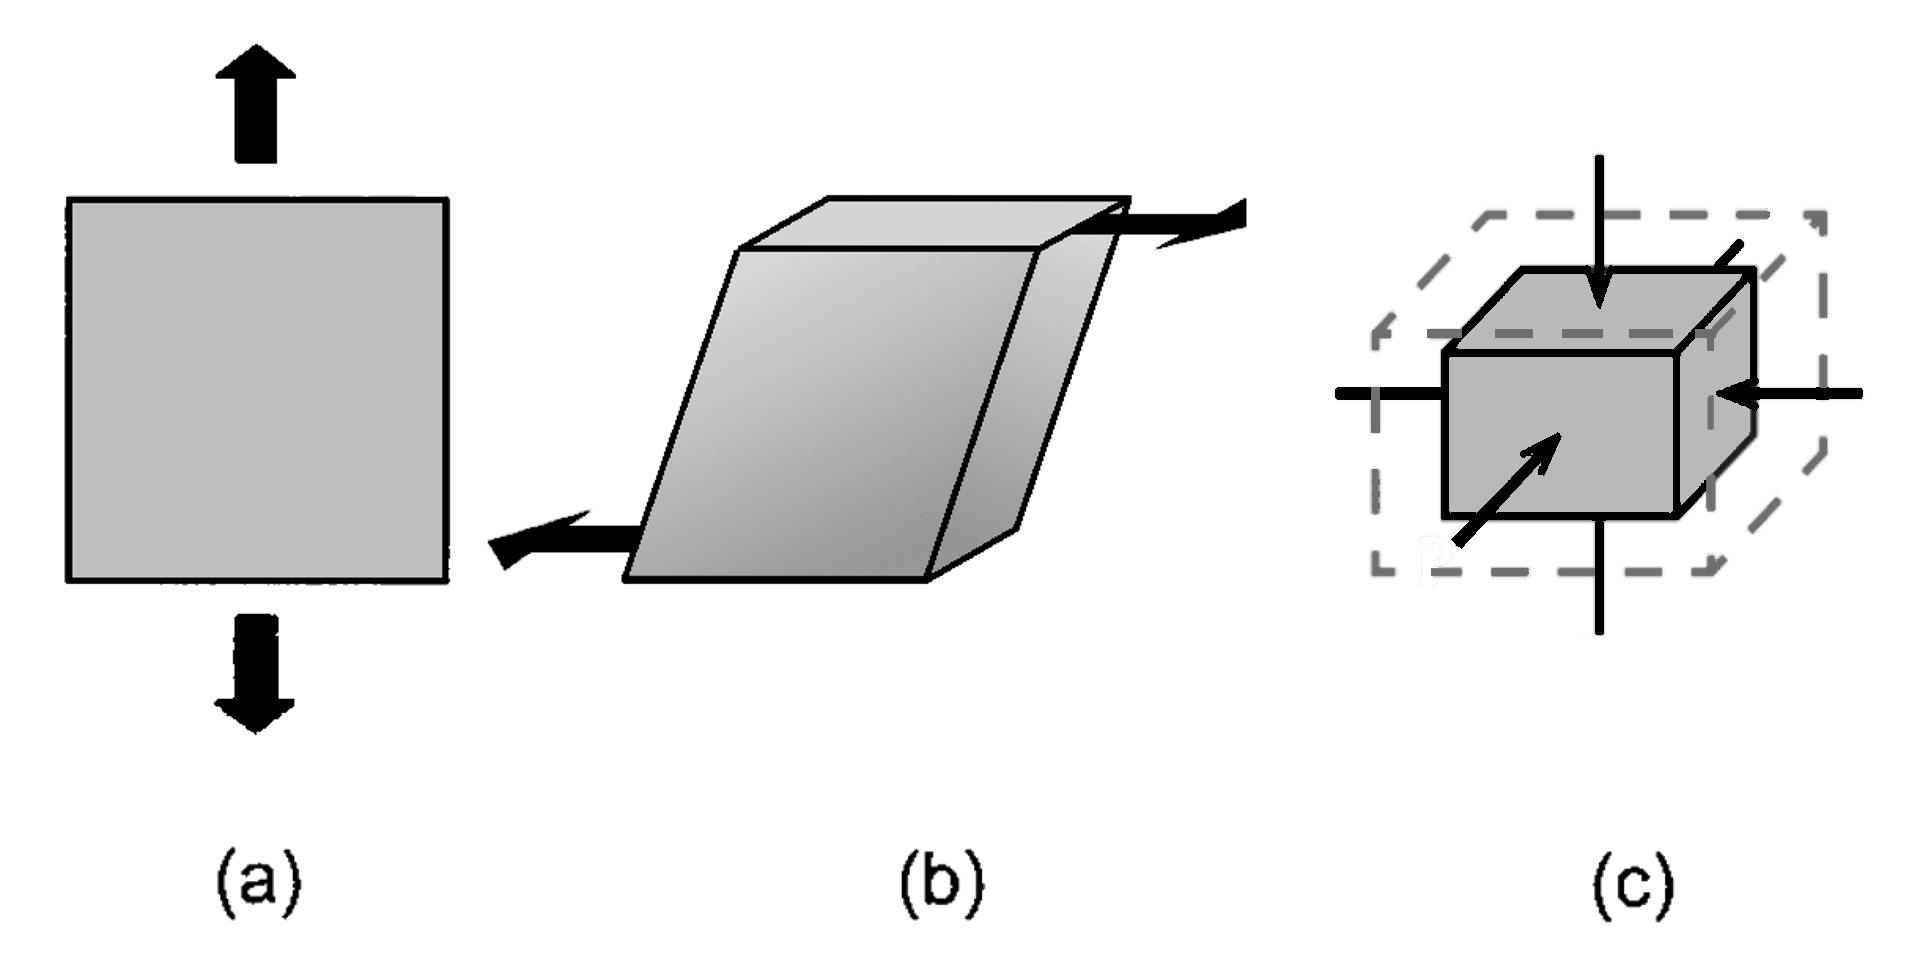
\includegraphics[width=0.7\linewidth]{obrazky/mechanical_tests}
		\caption[Mechanical tests to determine E, K, G moduli]{Mechanical tests to determine (a) E; (b) K; (c) G.}
		\label{fig:mechanicaltests}
	\end{figure}

	%%%%%%%%%%%%%%%%%%%%% SECOND LEVEL %%%%%%%%%%%%%%%%%%%%%%
	\item
	\textit{Second level}, where the constitutive equations must involve two (or more) additional variables. For instance:
	
	\begin{equation}\label{eq:second_level}
		f(\sigma,\varepsilon,\dot{\varepsilon},T)=0,
	\end{equation}
	
	where $\dot{\varepsilon}$ is the strain rate and $T$ is the temperature.
	These new variables are necessary for addition viscoelastic behavior into the material model. This behavior is linked to the molecular motions, which are important in the glassy domain, which between boundaries $\alpha$ and $\beta$ (in the map of Fig. \ref{fig:effectoncrosslinkdensity}). Also they affect the behavior in the glass transition region (around boundary $\alpha$). We also need relationships that describe the effects of $\dot{\varepsilon}$, $\dot{\sigma}$, and $T$ on the previously defined elastic properties. As next there will be required numerical boundary values of elastic properties, which are characterizing unrelaxed a relaxed states.
	
	\begin{figure}
		\centering
		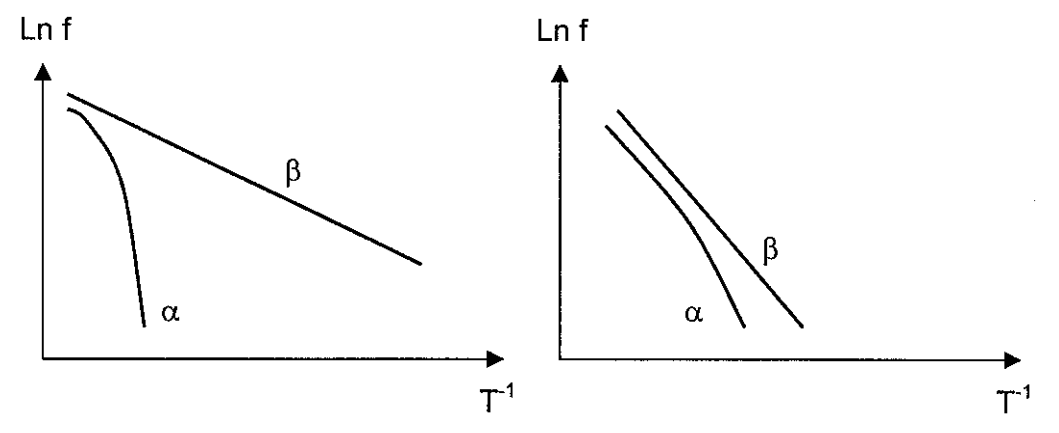
\includegraphics[width=0.8\linewidth]{obrazky/effect_on_cross_link_density}
		\caption[Shape of relaxation maps]{Shape of relaxation maps: In the figure you can see dependence of $\ln f$ (frequency) to reciprocal temperature for coordinates of transitions - $\alpha$, $\beta$: left - polymers having their $\alpha$ and $\beta$ transitions well separated; right - polymers with close $\alpha$ and $\beta$ transitions}
		\label{fig:effectoncrosslinkdensity}
	\end{figure}
	
	There we can find three major experimental methods for mechanical characterization in this region, which correspond to particular solutions of the material's state equation: 
	
	\begin{itemize}
		\item Static tests: $\varepsilon = \varepsilon_{0} = constant$ for relaxation or $\sigma = \sigma_{0} = constant$ for creep. 
		
		\item Monotonous tests with loading rate $\dot{\varepsilon}$ or $\dot{\sigma} = constant$ (for example tensile tests): 
		
		$\dot{\varepsilon} = \dfrac{1}{l}\dfrac{dl}{dt}$
		
		\item dynamic tests: $\varepsilon = \varepsilon_{0} \sin(\omega t)$ or $\sigma = \sigma_{0} \sin(\omega t)$
	\end{itemize}
	
	Polymers are generally assumed to obey the Boltzmann superposition principle in the region of small strains. When there are changes of loading conditions, the effects of these changes are additive when the corresponding responses are considered at equivalent times. For example, if different stresses $\sigma_{0}$, $\sigma_{1}$, $\sigma_{2}$,...$\sigma_{i}$ are applied at different times $0$, $t_{1}$, $t_{2}$,...$t_{i}$, respectively, the final strain is
	
	\begin{equation}\label{eq2:boltzmann_eps}
		\varepsilon(t) = J(t)\sigma_{0} + J(t-t_{1})\sigma_{1}+J(t-t_{2})\sigma_{2}+\cdots+J(t-t_{i})\sigma_{i}
	\end{equation}
	
	where $J(t)$ is the time-dependent creep compliance.
	
	In the same manner, if different strains $\varepsilon_{0}$, $\varepsilon_{1}$, $\varepsilon_{2}$,...$\varepsilon_{i}$ are applied at times $0$, $t_{1}$, $t_{2}$,...$t_{i}$, the final stress is 
	
	\begin{equation}\label{eq2:boltzmann_sig}
	\sigma(t) = E(t)\varepsilon_{0} + E(t-t_{1})\varepsilon_{1}+ E(t-t_{2})\varepsilon_{2}+\cdots+E(t-t_{i})\varepsilon_{i}
	\end{equation}
	
	where $E(t)$ is the time-dependent relaxation modulus. 
	
	Thats why we need to know $J(t)$ or $E(t)$. It is generally effective to use dynamic tests to obtain $J(\omega)$ or $E(\omega)$, and then, thanks to using mathematical transformations, determine $J(t)$ or $E(t)$.
	
	Ordinary, polymers obey a time-temperature superposition principle:
	
	\begin{equation}\label{eq2:shift_factor}
		P_{r}(t,T) = P_{r} \left(\dfrac{t}{a_{T}}, T_{r}\right)
	\end{equation}
	
	where $P_{r}$ is function of $T_{r}$ and $a_{t}$. In equation \ref{eq2:shift_factor} $T_{r}$ is reference temperature and $a_{T}$ is a shift factor, that dependence only on temperature. Polymers are interesting in that $a_{T} = f(T)$ witch take different mathematical forms below and above glass transition temperature $T_{g}$.
	
	%%%%%%%%%%%%%%%%%%%%% THIRD LEVEL %%%%%%%%%%%%%%%%%%%%%%
	\item
	\textit{Third level} of complexity, where is the unsteady character of the polymer linked to the fact, that it is out of equilibrium in the glassy state, and have to be taken into account. The behavior of the material does not depends only on the environmental conditions and mechanical stimulations but also on its thermo-mechanical history from its installation, which leads to adding the time variable to the constitutive equations:
	
	\begin{equation}
		f(\sigma,\varepsilon,\dot{\varepsilon},T,t)=0
	\end{equation}
	
	The adding time to the equation leads to add a effect called embrittlement to material behavior, which is decreasing in the fracture resistance by physical aging. Other aspect of mechanical behavior are not affected, or favorable by increase of relaxation times, decrease of creep or relaxation rates. For that reason are thermosets in most applications, by the knowledge of short-term properties, considered as sufficient for engineering design as far as durability and fracture are not concerned in model.
	
\end{itemize}


\subsection{Material properties}\label{subsec:mat_proper}
Material properties needed for studying long-term performance of thermosetting polymers include the kinetics reaction, associated curing degrees, viscoelastic properties, and standard mechanical properties, such as stiffness and fracture. And it is worth to mention that the degree of cure influences the glass-transition temperature, brittleness, impact resistance, creep behavior or long term stability and is dependent on both time and temperature. All of these i describe below in detail. 

\subsubsection{Standard mechanical properties}


There are two main sets of material properties involved in any problem of mechanical reliability\cite{thermosetting_polymers}.

\begin{itemize}
	\item \textit{Yielding properties.} Yielding or plastic deformation can be considered as the boundary between reversible and permanent deformation. In normal conditions, the material must be used below the yield boundary, often called elastic limit of material. 
	\item \textit{Fracture properties.} If the material goes beyond its yield boundary, becomes important the ultimate fracture stress or strain, where the integrity of the material is lost. Then we need specific theoretical and experimental tools, e.g., fracture mechanics, to study these phenomena. 
\end{itemize}



\subsection{Curing of adhesives}

\subsection{Viscoelastic properties}

\subsection{Numerical approximation}
